\documentclass[a4paper,11pt]{kth-mag}
\usepackage[T1]{fontenc}
\usepackage{textcomp}
\usepackage{lmodern}
\usepackage[utf8]{inputenc}
\usepackage[swedish,english]{babel}
\usepackage{modifications}

\usepackage{hyperref}
\hypersetup{colorlinks,citecolor=black,filecolor=black,linkcolor=black,urlcolor=black}

\usepackage{tikz}
\usetikzlibrary{positioning}

\title{Using binary decision diagrams to determine program equivalence in a superoptimizer}
\subtitle{}
\foreigntitle{Att använda binära beslutsdiagram för att avgöra ekvivalens mellan program i en superoptimerare}
\author{Jesper Särnesjö}
\date{}
\blurb{Master's Thesis at CSC \\ Supervisor: Torbjörn Granlund \\ Examiner: Johan Håstad}
\trita{TRITA xxx yyyy-nn}

\begin{document}

\frontmatter

\pagestyle{empty}

\removepagenumbers

\maketitle

\selectlanguage{english}

\begin{abstract}
\end{abstract}

\clearpage

\begin{foreignabstract}{swedish}
\end{foreignabstract}

\clearpage

\tableofcontents*

\mainmatter

\pagestyle{newchap}

\chapter{Introduction}

\chapter{Background}

\section{Superoptimizers}

A superoptimizer is a tool for finding the optimal program computing a given function.  % straight-line, loop-free
Typically, it takes as its input a description of a program, and yields as its output an equivalent, but optimal, program.
Here, two programs are considered equivalent if they always yield identical output given identical and valid input.

There are many possible measures of the optimality of a program.
The arguably simplest one is \emph{program length}, the number of instructions in the program.
Using this measure, a program is considered optimal if no equivalent program contains fewer instructions.
A similar measure is \emph{program size}, the number of bytes required to store the program. % difference only meaningful for variable instruction length architectures
Another measure is \emph{execution time}, the number of clock cycles it takes for the program to run from start to finish. % different and more complicated because...
The measures mentioned appear to be the ones used in practice, although any quantifiable property of a program could be used. % memory or power usage

The search strategy typically employed by superoptimizers, is to exhaustively generate potentially optimal candidate programs and test them for equivalence with the input program.
This works particularly well when the measure of optimality is program length, as the superoptimizer may then begin by generating and testing all programs of length 1, followed by those of length 2, and so on.
The first program found to be equivalent to the input program will necessarily be an optimal program.

It should be noted that exhaustive search over the space of all potentially optimal programs is very slow.
The number of programs of length $n$ using an instruction set consisting of $b$ instructions is $b^n$. % effective
For this reason, it is crucial to aggressively prune the search tree, ignoring programs which cannot possibly be optimal.

% determining equivalence

\subsection{History}

The term superoptimizer was coined by Henry Massalin in a paper published in 1987.
% Motorola 68020
% subset, no mem
% program length, exhaustive search
% equivalence tests: boolean -> 40/s, probabilistic -> 50k/s (executes code, host instruction set only)
% pruning: subsequence must also be optimal (only true for program size metric)
% applications
\cite{massalin87}

% GSO, the GNU superoptimizer
% like massalin: program length, probabilistic
% simulates instead of executes -> supports many architectures
% machine: registers + carry bit, no mem
% input: goal function compiled in
% pruning
% branching factor "between 100 and 1000"
% source code available
\cite{granlund92}

% Denali
% first publication in 2002
% execution time, provably correct equivalence, multiple assignments
% matcher
% solver
% input in somewhat C-like DSL
\cite{joshi02}

% Denali-2
% program length
% theoretical description of algo only, no implementation
\cite{joshi06}

% Bansal
% peephole superoptimizer
% fully automatic
% input: binary
% output: replacement rules
% execution time, program size
% x86
% pruning: meet-in-the-middle
% interesting application: binary translator
% source code available
\cite{bansal_thesis}

% TOAST, Total Optimisation using Answer Set Technology
\cite{crick_thesis}

\section{Binary decision diagrams}

Binary decision diagram (BDDs) are data structures used to efficiently represent a Boolean functions.
They consist of nodes, representing the function's variables. Each node has one or more incoming paths, and exactly two outgoing paths, commonly referred to as the \emph{high} and \emph{low} path.
When using a BDD to determine the value of a Boolean function, one follows a node's high path if its variable is 1, and it's low path if its variable is 0, starting at the root node, until one arrives at a terminal node.

BDDs were introduced by Lee \cite{lee59}, under the name \emph{binary-decision programs}.
They were given their current name by Akers \cite{akers78}, who also explored the ideas of \emph{reducing} BDDs by removing redundant nodes, and of representing multiple functions in a single BDD.

A more restricted type of BDD was introduced by Bryant \cite{bryant86}.
In addition to the above, Bryant required the BDD to be \emph{ordered}, having its variables appear in the same order on all paths from the root to a terminal node,
and to be \emph{reduced}, containing no node with the same high and low path, and no two distinct nodes with isomorphic subgraphs.
Such a BDD is called a \emph{reduced ordered BDD} (ROBDD), and has several beneficial characteristics.
First, the algorithms used to perform Boolean operations on one or a pair of ROBDDs, are efficient, requiring at worst a number of time steps proportial to the product of the number of nodes in the two ROBDDs.
Further, ROBDDs are \emph{canonical} representations of their Boolean functions, meaning that two Boolean functions are equivalent iff their ROBDDs are isomorphic.

Bryant also further explored the idea of representing multiple functions in a single BDD, which would later be referred to as a \emph{shared BDD} by Minato et al \cite{minato90}.
This type of BDD, the \emph{shared reduced ordered BDD} (SROBDD), has the added benefits of being memory efficient, and allowing an isomorphism test to be implemented as a single pointer comparison.

Bryant showed that the variable ordering used can have a dramatic effect on the number of nodes in a BDD, which in the best case is linear in the number of variables, and in the worst case exponential.
Further, finding the variable ordering which minimized the number of nodes is a coNP-complete problem. % proof? just say NP?

\subsection{Example}

To illustrate how a moderately complex Boolean function can be represented by a BDD, consider a class of functions with $2n$ variables labeled $a_0,...,a_{n-1},b_0,...,b_{n-1}$, defined recursively as follows:

$$
  c_k = \left\{
  \begin{array}{ll}
    a_k b_k                             & k = 0 \\
    a_k b_k + a_k c_{k-1} + b_k c_{k-1} & 0 < k < n \\
  \end{array}\right.
$$

$c_{n-1}$ is the function for the carry-out bit of an $n$-bit adder with no carry-in, taking $a$ and $b$ as its two inputs.
Its truth table is listed in Table~\ref{tab:tt_c1}, and it is shown in OBDD and ROBDD form in Figure~\ref{fig:bdd_c1}, using the variable ordering $a_0,b_0,...,a_{n-1},b_{n-1}$.
If we instead use the variable ordering $a_0,...,a_{n-1},b_0,...,b_{n-1}$, we end up with a larger ROBDD, as illustrated in Figure~\ref{fig:bdd_c2_bad}.
For this particular function, and these two variable orderings, the number of nodes required is:

$$
  |c_{n-1}| = \left\{
  \begin{array}{ll}
    3n-1      & \textrm{using variable order $a_0,b_0,...,a_{n-1},b_{n-1}$} \\
    2^{n+1}-2 & \textrm{using variable order $a_0,...,a_{n-1},b_0,...,b_{n-1}$} \\
  \end{array}\right.
$$

\begin{table}
\centering
\begin{tabular}{cccc|cc}
$a_0$ & $b_0$ & $a_1$ & $b_1$ & $c_0$ & $c_1$ \\
\hline
0     & 0     & 0     & 0     & 0     & 0 \\
0     & 0     & 0     & 1     & 0     & 0 \\
0     & 0     & 1     & 0     & 0     & 0 \\
0     & 0     & 1     & 1     & 0     & 1 \\
0     & 1     & 0     & 0     & 0     & 0 \\
0     & 1     & 0     & 1     & 0     & 0 \\
0     & 1     & 1     & 0     & 0     & 0 \\
0     & 1     & 1     & 1     & 0     & 1 \\
1     & 0     & 0     & 0     & 0     & 0 \\
1     & 0     & 0     & 1     & 0     & 0 \\
1     & 0     & 1     & 0     & 0     & 0 \\
1     & 0     & 1     & 1     & 0     & 1 \\
1     & 1     & 0     & 0     & 1     & 0 \\
1     & 1     & 0     & 1     & 1     & 1 \\
1     & 1     & 1     & 0     & 1     & 1 \\
1     & 1     & 1     & 1     & 1     & 1 \\
\end{tabular}
\caption{Truth table for the Boolean function $c_1$.}
\label{tab:tt_c1}
\end{table}

\begin{figure}
\centering
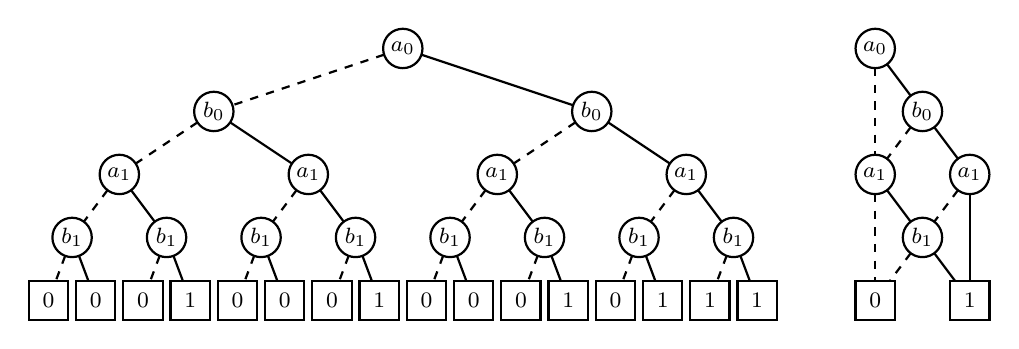
\begin{tikzpicture}
[every node/.style={draw=black,thick,minimum size=5mm,inner sep=0mm,outer sep=0mm,font=\footnotesize},
 var/.style={circle},
 val/.style={rectangle},
 thick]
\node[var] (a0)                                            {$a_0$};
\node[var] (b0A) [on grid,below  left=8mm and 24mm of a0]  {$b_0$};
\node[var] (b0B) [on grid,below right=8mm and 24mm of a0]  {$b_0$};
\node[var] (a1A) [on grid,below  left=8mm and 12mm of b0A] {$a_1$};
\node[var] (a1B) [on grid,below right=8mm and 12mm of b0A] {$a_1$};
\node[var] (a1C) [on grid,below  left=8mm and 12mm of b0B] {$a_1$};
\node[var] (a1D) [on grid,below right=8mm and 12mm of b0B] {$a_1$};
\node[var] (b1A) [on grid,below  left=8mm and  6mm of a1A] {$b_1$};
\node[var] (b1B) [on grid,below right=8mm and  6mm of a1A] {$b_1$};
\node[var] (b1C) [on grid,below  left=8mm and  6mm of a1B] {$b_1$};
\node[var] (b1D) [on grid,below right=8mm and  6mm of a1B] {$b_1$};
\node[var] (b1E) [on grid,below  left=8mm and  6mm of a1C] {$b_1$};
\node[var] (b1F) [on grid,below right=8mm and  6mm of a1C] {$b_1$};
\node[var] (b1G) [on grid,below  left=8mm and  6mm of a1D] {$b_1$};
\node[var] (b1H) [on grid,below right=8mm and  6mm of a1D] {$b_1$};
\node[val] (tA)  [on grid,below  left=8mm and  3mm of b1A] {0};
\node[val] (tB)  [on grid,below right=8mm and  3mm of b1A] {0};
\node[val] (tC)  [on grid,below  left=8mm and  3mm of b1B] {0};
\node[val] (tD)  [on grid,below right=8mm and  3mm of b1B] {1};
\node[val] (tE)  [on grid,below  left=8mm and  3mm of b1C] {0};
\node[val] (tF)  [on grid,below right=8mm and  3mm of b1C] {0};
\node[val] (tG)  [on grid,below  left=8mm and  3mm of b1D] {0};
\node[val] (tH)  [on grid,below right=8mm and  3mm of b1D] {1};
\node[val] (tI)  [on grid,below  left=8mm and  3mm of b1E] {0};
\node[val] (tJ)  [on grid,below right=8mm and  3mm of b1E] {0};
\node[val] (tK)  [on grid,below  left=8mm and  3mm of b1F] {0};
\node[val] (tL)  [on grid,below right=8mm and  3mm of b1F] {1};
\node[val] (tM)  [on grid,below  left=8mm and  3mm of b1G] {0};
\node[val] (tN)  [on grid,below right=8mm and  3mm of b1G] {1};
\node[val] (tO)  [on grid,below  left=8mm and  3mm of b1H] {1};
\node[val] (tP)  [on grid,below right=8mm and  3mm of b1H] {1};
\path[dashed] (a0)  edge (b0A);
\path         (a0)  edge (b0B);
\path[dashed] (b0A) edge (a1A);
\path         (b0A) edge (a1B);
\path[dashed] (b0B) edge (a1C);
\path         (b0B) edge (a1D);
\path[dashed] (a1A) edge (b1A);
\path         (a1A) edge (b1B);
\path[dashed] (a1B) edge (b1C);
\path         (a1B) edge (b1D);
\path[dashed] (a1C) edge (b1E);
\path         (a1C) edge (b1F);
\path[dashed] (a1D) edge (b1G);
\path         (a1D) edge (b1H);
\path[dashed] (b1A) edge (tA);
\path         (b1A) edge (tB);
\path[dashed] (b1B) edge (tC);
\path         (b1B) edge (tD);
\path[dashed] (b1C) edge (tE);
\path         (b1C) edge (tF);
\path[dashed] (b1D) edge (tG);
\path         (b1D) edge (tH);
\path[dashed] (b1E) edge (tI);
\path         (b1E) edge (tJ);
\path[dashed] (b1F) edge (tK);
\path         (b1F) edge (tL);
\path[dashed] (b1G) edge (tM);
\path         (b1G) edge (tN);
\path[dashed] (b1H) edge (tO);
\path         (b1H) edge (tP);
\node[var] (Ra0)  [on grid,right=60 mm of a0]               {$a_0$};
\node[var] (Rb0)  [on grid,below right=8mm and 6mm of Ra0]  {$b_0$};
\node[var] (Ra1A) [on grid,below  left=8mm and 6mm of Rb0]  {$a_1$};
\node[var] (Ra1B) [on grid,below right=8mm and 6mm of Rb0]  {$a_1$};
\node[var] (Rb1)  [on grid,below right=8mm and 6mm of Ra1A] {$b_1$};
\node[val] (R0)   [on grid,below  left=8mm and 6mm of Rb1]  {0};
\node[val] (R1)   [on grid,below right=8mm and 6mm of Rb1]  {1};
\path[dashed] (Ra0)  edge (Ra1A);
\path         (Ra0)  edge (Rb0);
\path[dashed] (Rb0)  edge (Ra1A);
\path         (Rb0)  edge (Ra1B);
\path[dashed] (Ra1A) edge (R0);
\path         (Ra1A) edge (Rb1);
\path[dashed] (Ra1B) edge (Rb1);
\path         (Ra1B) edge (R1);
\path[dashed] (Rb1)  edge (R0);
\path         (Rb1)  edge (R1);
\end{tikzpicture}
\caption{The Boolean function $c_1$ as an OBDD (left) and an ROBDD (right). The solid lines represent high paths and the dashed lines represent low paths.}
\label{fig:bdd_c1}
\end{figure}

\begin{figure}
\centering
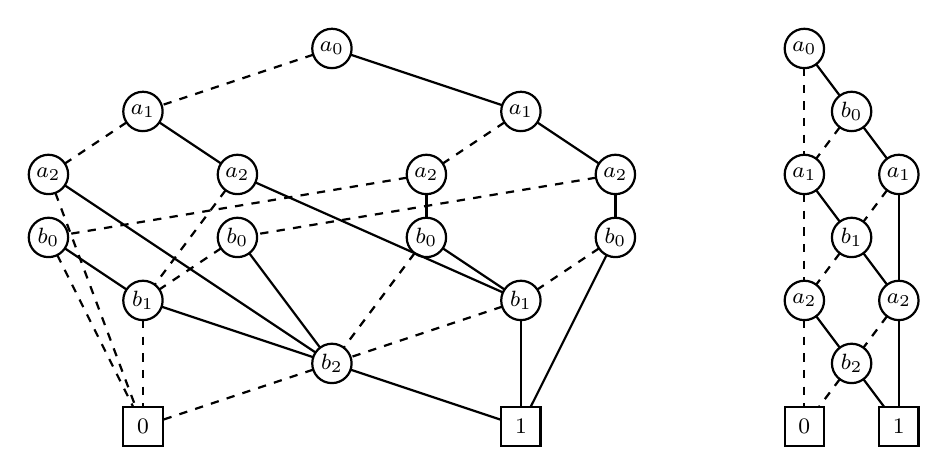
\begin{tikzpicture}
[every node/.style={draw=black,thick,minimum size=5mm,inner sep=0mm,outer sep=0mm,font=\footnotesize},
 var/.style={circle},
 val/.style={rectangle},
 thick]
\node[var] (a0)                                            {$a_0$};
\node[var] (a1A) [on grid,below  left=8mm and 24mm of a0]  {$a_1$};
\node[var] (a1B) [on grid,below right=8mm and 24mm of a0]  {$a_1$};
\node[var] (a2A) [on grid,below  left=8mm and 12mm of a1A] {$a_2$};
\node[var] (a2B) [on grid,below right=8mm and 12mm of a1A] {$a_2$};
\node[var] (a2C) [on grid,below  left=8mm and 12mm of a1B] {$a_2$};
\node[var] (a2D) [on grid,below right=8mm and 12mm of a1B] {$a_2$};
\node[var] (b0A) [on grid,below right=8mm and  0mm of a2A] {$b_0$};
\node[var] (b0B) [on grid,below right=8mm and  0mm of a2B] {$b_0$};
\node[var] (b0C) [on grid,below right=8mm and  0mm of a2C] {$b_0$};
\node[var] (b0D) [on grid,below right=8mm and  0mm of a2D] {$b_0$};
\node[var] (b1A) [on grid,below right=8mm and 12mm of b0A] {$b_1$};
\node[var] (b1B) [on grid,below right=8mm and 12mm of b0C] {$b_1$};
\node[var] (b2)  [on grid,below right=8mm and 24mm of b1A] {$b_2$};
\node[val] (0)   [on grid,below  left=8mm and 24mm of b2]  {0};
\node[val] (1)   [on grid,below right=8mm and 24mm of b2]  {1};
\path[dashed] (a0)  edge (a1A);
\path         (a0)  edge (a1B);
\path[dashed] (a1A) edge (a2A);
\path         (a1A) edge (a2B);
\path[dashed] (a1B) edge (a2C);
\path         (a1B) edge (a2D);
\path[dashed] (a2A) edge (0);
\path         (a2A) edge (b2);
\path[dashed] (a2B) edge (b1A);
\path         (a2B) edge (b1B);
\path[dashed] (a2C) edge (b0A);
\path         (a2C) edge (b0C);
\path[dashed] (a2D) edge (b0B);
\path         (a2D) edge (b0D);
\path[dashed] (b0A) edge (0);
\path         (b0A) edge (b1A);
\path[dashed] (b0B) edge (b1A);
\path         (b0B) edge (b2);
\path[dashed] (b0C) edge (b2);
\path         (b0C) edge (b1B);
\path[dashed] (b0D) edge (b1B);
\path         (b0D) edge (1);
\path[dashed] (b1A) edge (0);
\path         (b1A) edge (b2);
\path[dashed] (b1B) edge (b2);
\path         (b1B) edge (1);
\path[dashed] (b2)  edge (0);
\path         (b2)  edge (1);
\node[var] (Ga0)  [on grid,right=60mm of a0]                {$a_0$};
\node[var] (Gb0)  [on grid,below right=8mm and 6mm of Ga0]  {$b_0$};
\node[var] (Ga1A) [on grid,below  left=8mm and 6mm of Gb0]  {$a_1$};
\node[var] (Ga1B) [on grid,below right=8mm and 6mm of Gb0]  {$a_1$};
\node[var] (Gb1)  [on grid,below right=8mm and 6mm of Ga1A] {$b_1$};
\node[var] (Ga2A) [on grid,below  left=8mm and 6mm of Gb1]  {$a_2$};
\node[var] (Ga2B) [on grid,below right=8mm and 6mm of Gb1]  {$a_2$};
\node[var] (Gb2)  [on grid,below right=8mm and 6mm of Ga2A] {$b_2$};
\node[val] (G0)   [on grid,below  left=8mm and 6mm of Gb2]  {0};
\node[val] (G1)   [on grid,below right=8mm and 6mm of Gb2]  {1};
\path[dashed] (Ga0)  edge (Ga1A);
\path         (Ga0)  edge (Gb0);
\path[dashed] (Gb0)  edge (Ga1A);
\path         (Gb0)  edge (Ga1B);
\path[dashed] (Ga1A) edge (Ga2A);
\path         (Ga1A) edge (Gb1);
\path[dashed] (Ga1B) edge (Gb1);
\path         (Ga1B) edge (Ga2B);
\path[dashed] (Gb1)  edge (Ga2A);
\path         (Gb1)  edge (Ga2B);
\path[dashed] (Ga2A) edge (G0);
\path         (Ga2A) edge (Gb2);
\path[dashed] (Ga2B) edge (Gb2);
\path         (Ga2B) edge (G1);
\path[dashed] (Gb2)  edge (G0);
\path         (Gb2)  edge (G1);
\end{tikzpicture}
\caption{The Boolean function $c_2$ in ROBDD form using the variable order $a_0,a_1,a_2,b_0,b_1,b_2$ (left) and $a_0,b_0,a_1,b_1,a_2,b_2$ (right).}
\label{fig:bdd_c2_bad}
\end{figure}

\chapter{...}

% machine: registers,flags

\section{...}

\subsection{Flag control}

% stc,clc,cmc

\subsection{Data transfer}

% mov,cmov

\subsection{Logic}

% and,or,xor
% not (one's complement negation)

\subsection{Addition and subtraction}

% add
% adc,sub,sbb,cmp,inc,dec all similar
% neg (two's complement negation): not+inc

\subsection{Multiplication}

% most difficult: multiplication

\bibliographystyle{ieeetr}
\bibliography{thesis}

\appendix
\addappheadtotoc

\end{document}
